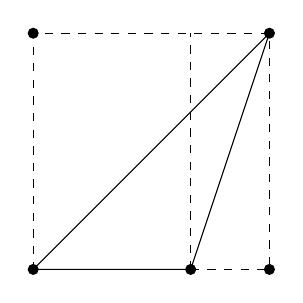
\begin{tikzpicture}

\coordinate (A) at (-2, 0);
% \node at (A) [below]{$A$};
\fill (A)  circle[radius=2pt];

\coordinate (B) at (0,0);
% \node at (B) [below]{$B$};
\fill (B)  circle[radius=2pt];

\coordinate (C) at (1,3);
% \node at (C) [above]{$C$};
\fill (C)  circle[radius=2pt];

\coordinate (D) at (-2,3);
% \node at (D) [above]{$D$};
\fill (D)  circle[radius=2pt];

\coordinate (E) at (1,0);
% \node at (E) [above]{$E$};
\fill (E)  circle[radius=2pt];


\draw (A) -- (B) -- (C) -- (A); 
\draw [,dashed] (B) -- (E) -- (C) -- (D) -- (A);
\draw [dashed] (B) -- (0,3);


\end{tikzpicture}